\documentclass[9pt]{beamer}

\usepackage[utf8x]{inputenc}

\usetheme{Ampang}
%%% XeLaTeX engine for Ubuntu Font support
\usepackage{xltxtra}
\usepackage{tikz}
\setsansfont[
BoldFont=Ubuntu-Bold.ttf,
ItalicFont=Ubuntu-Italic.ttf,
BoldItalicFont=Ubuntu-BoldItalic.ttf
]
{UbuntuMono-Regular.ttf}
\setmonofont{UbuntuMono-Regular.ttf}

\newcommand\Wider[2][3em]{%
\makebox[\linewidth][c]{%
  \begin{minipage}{\dimexpr\textwidth+#1\relax}
  \raggedright#2
  \end{minipage}%
  }%
}

\newcommand{\BackgroundImage}[2][0.3] {
  \tikz[remember picture,overlay]
  \node[opacity=#1, inner sep=0pt] at (current page.center)
       {\includegraphics[width=\paperwidth,height=\paperheight]{#2}};
       \clearpage
}

\title{Return Oriented Program Evolution with ROPER}
\author{Olivia Lucca Fraser}

\institute{NIMS Lab, Dalhousie University}

\begin{document}

%\maketitle


\begin{frame}%{\theframenumber. Overview}

  \BackgroundImage[0.2]{../images/roper.png}

  \begin{columns}
    \begin{column}{.5\textwidth}
     %
\includegraphics[width=\textwidth]{../images/roper.png} 
      {\Huge 
        \begin{tabular}{l}
          \texttt{R\,E\,T\,U\,R\,N} \\ 
          \texttt{O\,R\,I\,E\,N\,T\,E\,D} \\
          \texttt{P\,R\,O\,G\,R\,A\,M\,M\,E} \\
          \texttt{E\,V\,O\,L\,U\,T\,I\,O\,N}~{\large \texttt{with}} \\
          \texttt{R\,O\,P\,E\,R} \\
          \\
          \\
          \\
        \end{tabular}
      }
      {\large
        \begin{tabular}{l}
          \\
          \texttt{Olivia Lucca Fraser} \\
          \url{oluccafraser@tenable.com} \\
          \url{https://github.com/oblivia-simplex} \\
          \texttt{AtlSecCon, Halifax, April 28, 2017} \\
          \\
          \\
        \end{tabular}
      }
    \end{column}
    \begin{column}{.5\textwidth}
      %\begin{itemize}
      %\item What is Return Oriented Programming?
      %\item What is Genetic Programming?
      %\item How 
      %\end{itemize}
    \end{column}
  \end{columns}
\end{frame}

\begin{frame}%{\theframenumber. Overview}
  \BackgroundImage[0.2]{../images/roper.png}
  \begin{columns}
    \begin{column}{.5\textwidth}
     %
\includegraphics[width=\textwidth]{../images/roper.png} 
      {\Huge 
        \begin{tabular}{l}
          \texttt{R\,E\,T\,U\,R\,N} \\ 
          \texttt{O\,R\,I\,E\,N\,T\,E\,D} \\
          \texttt{P\,R\,O\,G\,R\,A\,M\,M\,E} \\
          \texttt{E\,V\,O\,L\,U\,T\,I\,O\,N}~{\large \texttt{with}} \\
          \texttt{R\,O\,P\,E\,R} \\
          \\
          \\
          \\
        \end{tabular}
      }
      {\large
        \begin{tabular}{l}
          \\
          \\ %\texttt{Olivia Lucca Fraser} \\
          \\ %\url{oluccafraser@tenable.com} \\
          \\ %\url{https://github.com/oblivia-simplex} \\
          \\ %\texttt{AtlSecCon, Halifax, April 28, 2017} \\
          \\
          \\
        \end{tabular}
      }
    \end{column}
    \begin{column}{.5\textwidth}

      \vspace{80pt}
      
      {\Large ~Questions: }
      \begin{itemize}
      \item What is return oriented programming?
      \item What is genetic programming?
      \item How do we best cultivate the evolution of ROP payloads?
      \item What sort of things are they capable of? 

      \end{itemize}
    \end{column}
  \end{columns}
\end{frame}

\begin{frame}{\theframenumber. A Quick Introduction to Return Oriented Programming}
  \begin{columns}
    \begin{column}{.4\textwidth}
      
\includegraphics[width=\textwidth]{../images/macgyver-transparent.png}
    \end{column}
    \begin{column}{.6\textwidth}
      \begin{itemize}
      \item SITUATION: You have found an exploitable vulnerability in a target process, and are able to corrupt the instruction pointer.
        \item PROBLEM: The system or process enforces $W\oplus X$: you can't write to executable memory, and you can't execute writeable memory. Old-school shellcode attacks won't work. 
        \item SOLUTION: You can't introduce any code of your own, but you \emph{can} reuse little `gadgets' of code that have already been mapped to executable memory. The trick is rearranging these gadgets into something useful.
      \end{itemize}
    \end{column}
    \end{columns}
\end{frame}

\begin{frame}{\theframenumber. What is a ROP chain?}

  \BackgroundImage[0.15]{../images/macgyver2-transparent.png}

  \begin{columns}
    \begin{column}{.5\textwidth}
      \begin{itemize}
      \item A `gadget' is any chunk of machine code that
        
        \begin{enumerate}
        \item[1.] is already mapped to executable memory
        \item[2.] allows us to regain control of the instruction pointer after it executes
        \end{enumerate}

      \item The way a ROP gadget lets us regain control is that it ends with a particular form of RETURN statement -- those that pop an address off the stack into the instruction pointer.  
      \item Ordinarily, the address popped from the stack is a `bookmark' pointing to the site in the code from which a function was called...
      \end{itemize}

    \end{column}
    \begin{column}{.5\textwidth}
      \begin{itemize}
      \item ...but this is just a convention. If an instruction pops an address from the stack into the IP, it will do so no matter \emph{what} address we put there.
      \item and we can take advantage of this to `chain' arbitrarily many gadgets together. As each reaches its RETURN instruction, it sends the instruction pointer to the next gadget in the chain.
      \end{itemize}
    \end{column}
  \end{columns}


\end{frame}


\begin{frame}{\theframenumber. An Equally Quick Introduction to Genetic Programming}


  \tikz[remember picture,overlay]
  \node[opacity=0.6, inner sep=0pt] at (current page.center)
       {
\includegraphics[width=\paperwidth,height=\paperheight]{../images/AI_ooze_transparent.png}};
       \clearpage

%  
\includegraphics[width=\textwidth]{../images/AI_ooze_transparent.png}
  \begin{columns}
    \begin{column}{.5\textwidth}
      What is necessary in order for natural selection to take place?
      \begin{enumerate}
      \item Reproduction with mutation 
      \item Variation in performance
      \item Selection by performance
      \end{enumerate}
      Anything that implements these traits can implement Darwinian evolution. 
    \end{column}
    \begin{column}{.5\textwidth}
      % will appear on mulder's mouth % Including malware?
    \end{column}
    \end{columns}
\end{frame}


\begin{frame}{\theframenumber. How ROPER works}

  \BackgroundImage[0.7]{../images/simplefarmer.png}
  \begin{columns}
    \begin{column}{.5\textwidth}
    \end{column}
    \begin{column}{.5\textwidth}

    \end{column}
    \end{columns}
\end{frame}

\begin{frame}{\theframenumber. Evolutionary computation}
  \begin{columns}
    \begin{column}{.5\textwidth}
      The idea of implementing evolution in code is almost as old as modern computing itself.
      \vspace{8pt}

      [POTTED HISTORY / TIMELINE]



      The variety of evolutionary computation implemented by ROPER closely approximates linear genetic programming, with a few crucial differences.

    \end{column}
    \begin{column}{.5\textwidth}

      A high-level outline of the algorithm it implements:
      \begin{enumerate}
      \item a set of gadgets is harvested from the target binary
      \item an initial, random population of chains is generated
      \item until a specified goal is achieved:
        \begin{enumerate}
        \item $n$ chains are selected at random
        \item they are executed in a VM, and their behaviour is assessed for fitness
        \item the fittest two chains are chosen to mate
        \item and their offspring are inserted into the population
        \item replacing the least fit chains in the competition
        \end{enumerate}
      \end{enumerate}
    \end{column}
  \end{columns}
\end{frame}

\begin{frame}{\theframenumber. Architecture of ROPER}
  %% ROPER's pattern matching functionality
      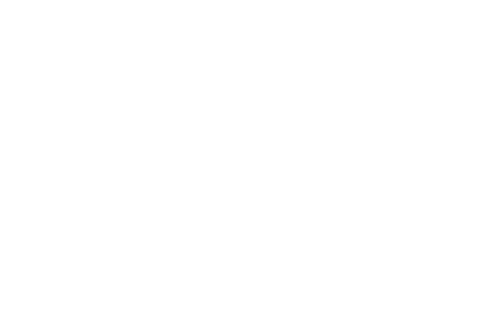
\includegraphics[width=\textwidth]{../images/architecture-transparent.png}
\end{frame}

\begin{frame}{\theframenumber. Pattern matching}
  \begin{columns}
    \begin{column}{.5\textwidth}
      The most basic type of problem that ROPER can breed a population of chains to solve is that achieving a determinate register state in the CPU, specified by a simple pattern consisting of integers and wildcards.
      \vspace{8pt}

      This isn't the most intriguing thing that ROPER can do, but it is fairly useful, automating the ordinary, human task of assembling a ROP chain that prepares the CPU for a system call -- to spawn a process, write to a file, open a socket, etc.
    \end{column}
    \begin{column}{.5\textwidth}
      For example, suppose we wanted to prime the CPU for the call
      $$\texttt{execv("/bin/sh", ["/bin/sh"], 0);}$$
      We'd need a ROP chain that sets \texttt{r0} and \texttt{r1} to point to some memory location that contains \texttt{"/bin/sh"}, sets \texttt{r2} to 0, and \texttt{r7} to 11. Once that's in place spawning a shell is as simple as jumping to any given address that contains an \texttt{svc} instruction.
      \vspace{8pt}

      One of ROPER's more peculiar solutions to this problem -- using gadgets from a Tomato router's HTTP daemon -- is on the next slide...
    \end{column}
  \end{columns}
\end{frame}

\begin{frame}{} %{\theframenumber. Strange Paths \& Dark Gadgets}
\begin{center}
  
    {\tiny
      \begin{tabular}{l l l} \hline
        \textbf{\texttt{;; Gadget 0}} 			& \textbf{\texttt{;; Deep Gadget 0}}				& \textbf{\texttt{;; Deep Gadget 1}} \\ 
        \texttt{[000100fc]  mov r0, r6} 	& \texttt{[00016890]  str r0, [r4, \#0x1c]}		& \texttt{[00012780]  bne \#0x18} \\
        \texttt{[00010100]  ldrb r4, [r6], \#1} & \texttt{[00016894]  mov r0, r4}		& \texttt{[00012784]  add r5, r5, r7} \\
        \texttt{[00010104]  cmp r4, \#0}	& \texttt{[00016898]  pop \{r4, lr\}}			& \texttt{[00012788]  rsb r4, r7, r4} \\
        \texttt{[00010108]  bne \#4294967224} & \texttt{[0001689c]  b \#4294966744}	& \texttt{[0001278c]  cmp r4, \#0} \\
        \texttt{[0001010c]  rsb r5, r5, r0}	& \texttt{[00016674]  push \{r4, lr\}}		& \texttt{[00012790]  bgt \#4294967240} \\
        \texttt{[00010110]  cmp r5, \#0x40} & \texttt{[00016678]  mov r4, r0}		& \texttt{[00012794]  b \#8} \\
        \texttt{[00010114]  movgt r0, \#0}	& \texttt{[0001667c]  ldr r0, [r0, \#0x18]}	& \texttt{[0001279c]  mov r0, r7} \\
        \texttt{[00010118]  movle r0, \#1}	& \texttt{[00016680]  ldr r3, [r4, \#0x1c]}	& \texttt{[000127a0]  pop \{r3, r4, r5, r6, r7, pc\}} \\
        \texttt{[0001011c]  pop \{r4, r5, r6, pc\}} & \texttt{[00016684]  cmp r0, \#0}		& \\
 				& \texttt{[00016688]  ldrne r1, [r0, \#0x20]}	& \texttt{R0: 0002bc3e} \\
        \texttt{R0: 00000001} 			& \texttt{[0001668c]  moveq r1, r0}		& \texttt{R1: 00000000} \\
        \texttt{R1: 00000001} 			& \texttt{[00016690]  cmp r3, \#0}		& \texttt{R2: 00000000} \\
        \texttt{R2: 00000001} 			& \texttt{[00016694]  ldrne r2, [r3, \#0x20]}	& \texttt{R7: 0000000b} \\
        \texttt{R7: 0002bc3e} 			& \texttt{[00016698]  moveq r2, r3}		& \\
        & \texttt{[0001669c]  rsb r2, r2, r1}		& \texttt{;; Deep Gadget 2} \\
        \textbf{\texttt{;; Gadget 1}} 		& \texttt{[000166a0]  cmn r2, \#1}		& \texttt{[000155ec]  b \#0x1c} \\
        \texttt{[00012780]  bne \#0x18}	& \texttt{[000166a4]  bge \#0x48}			& \texttt{[00015608]  add sp, sp, \#0x58} \\
        \texttt{[00012798]  mvn r7, \#0}	& \texttt{[000166ec]  cmp r2, \#1}			& \texttt{[0001560c]  pop \{r4, r5, r6, pc\}} \\
        \texttt{[0001279c]  mov r0, r7}	& \texttt{[000166f0]  ble \#0x44}			& \\
        \texttt{[000127a0]  pop \{r3, r4, r5, r6, r7, pc\}} & \texttt{[00016734]  mov r2, \#0} & \texttt{R0: 0002bc3e} \\
 				& \texttt{[00016738]  cmp r0, r2}			& \texttt{R1: 00000000} \\
        \texttt{R0: ffffffff}			& \texttt{[0001673c]  str r2, [r4, \#0x20]}		& \texttt{R2: 00000000} \\
        \texttt{R1: 00000001}		& \texttt{[00016740]  beq \#0x10}			& \texttt{R7: 0000000b} \\
        \texttt{R2: 00000001}		& \texttt{[00016750]  cmp r3, \#0}			& \\
        \texttt{R7: ffffffff}			& \texttt{[00016754]  beq \#0x14}			& \textbf{\texttt{;; Deep Gadget 3}} \\
 					& \texttt{[00016758]  ldr r3, [r3, \#0x20]}	& \texttt{[00016918]  mov r1, r5   **}\\
        \textbf{\texttt{;; Gadget 2}}		& \texttt{[0001675c]  ldr r2, [r4, \#0x20]}		& \texttt{[0001691c]  mov r2, r6} \\
        \texttt{[00016884]  beq \#0x1c}	& \texttt{[00016760]  cmp r3, r2}			& \texttt{[00016920]  bl \#4294967176} \\
        \texttt{[00016888]  ldr r0, [r4, \#0x1c]} & \texttt{[00016764]  strgt r3, [r4, \#0x20]} & \texttt{[000168a8]  push \{r4, r5, r6, r7, r8, lr\}} \\
        \texttt{[0001688c]  bl \#4294967280} & \texttt{[00016768]  ldr r3, [r4, \#0x20]}	& \texttt{[000168ac]  subs r4, r0, \#0} \\
        \texttt{[0001687c]  push \{r4, lr\}}	& \texttt{[0001676c]  mov r0, r4}		& \texttt{[000168b0]  mov r5, r1} \\
        \texttt{[00016880]  subs r4, r0, \#0} & \texttt{[00016770]  add r3, r3, \#1}		& \texttt{[000168b4]  mov r6, r2} \\
        \texttt{[00016884]  beq \#0x1c}	& \texttt{[00016774]  str r3, [r4, \#0x20]}		& \texttt{[000168b8]  beq \#0x7c} \\
        \texttt{[000168a0]  mov r0, r1}	& \texttt{[00016778]  pop \{r4, pc\}}			& \texttt{[000168bc]  mov r0, r1} \\
        \texttt{[000168a4]  pop \{r4, pc\}}	&							& \texttt{[000168c0]  mov r1, r4} \\
 					&							& \texttt{[000168c4]  blx r2} \\
\texttt{R0: 00000001}			& \texttt{R0: 0000000b}				& \\
\texttt{R1: 00000001}			& \texttt{R1: 00000000}				& \texttt{R0: 0002bc3e} \\
\texttt{R2: 00000001}			& \texttt{R2: 00000000}				& \texttt{R1: 0002bc3e} \\
\texttt{R7: 0002bc3e}				& \texttt{R7: 0002bc3e}				& \texttt{R2: 00000000} \\
					&							& \texttt{R7: 0000000b} \\ \hline
      \end{tabular}
    }
    
\end{center}
\end{frame}

\begin{frame}{\theframenumber. Deep Gadgets, Introns, \& Extended Phenotypes}
  \BackgroundImage[0.15]{../images/exons.png}
  \begin{columns}


    \begin{column}{.5\textwidth}
      What makes this chain so interesting is that its execution path -- its
      `behavioural phenotype' -- spends most of its time in gadgets that aren't
      referenced in the chain itself (labelled `deep gadgets' on the last
      slide). This is because gadget \#\,2 jumps backwards, writes to its own
      call stack, and overrides the pointers in its own genome.
      \vspace{8pt}

      Chains like this emerge frequently from ROPER's populations, and are usually accompanied by spikes in the population's crash frequency -- jumping blindly to arbitrary addresses is hazardous.
      \vspace{8pt}


    \end{column}

    \begin{column}{.5\textwidth}
      What selection pressures could be responsible for this phenomenon? There
      is, after all, a moderate fitness penalty for chains that crash (which
      reduces their chances of breeding).
      \vspace{8pt}

      The reason I conjecture is that these chains 
    \end{column}
  \end{columns}
\end{frame}



\begin{frame}{\theframenumber. Fleurs du Malware }

  \tikz[remember picture,overlay]
  \node[opacity=0.3, inner sep=0pt] at (current page.center)
       {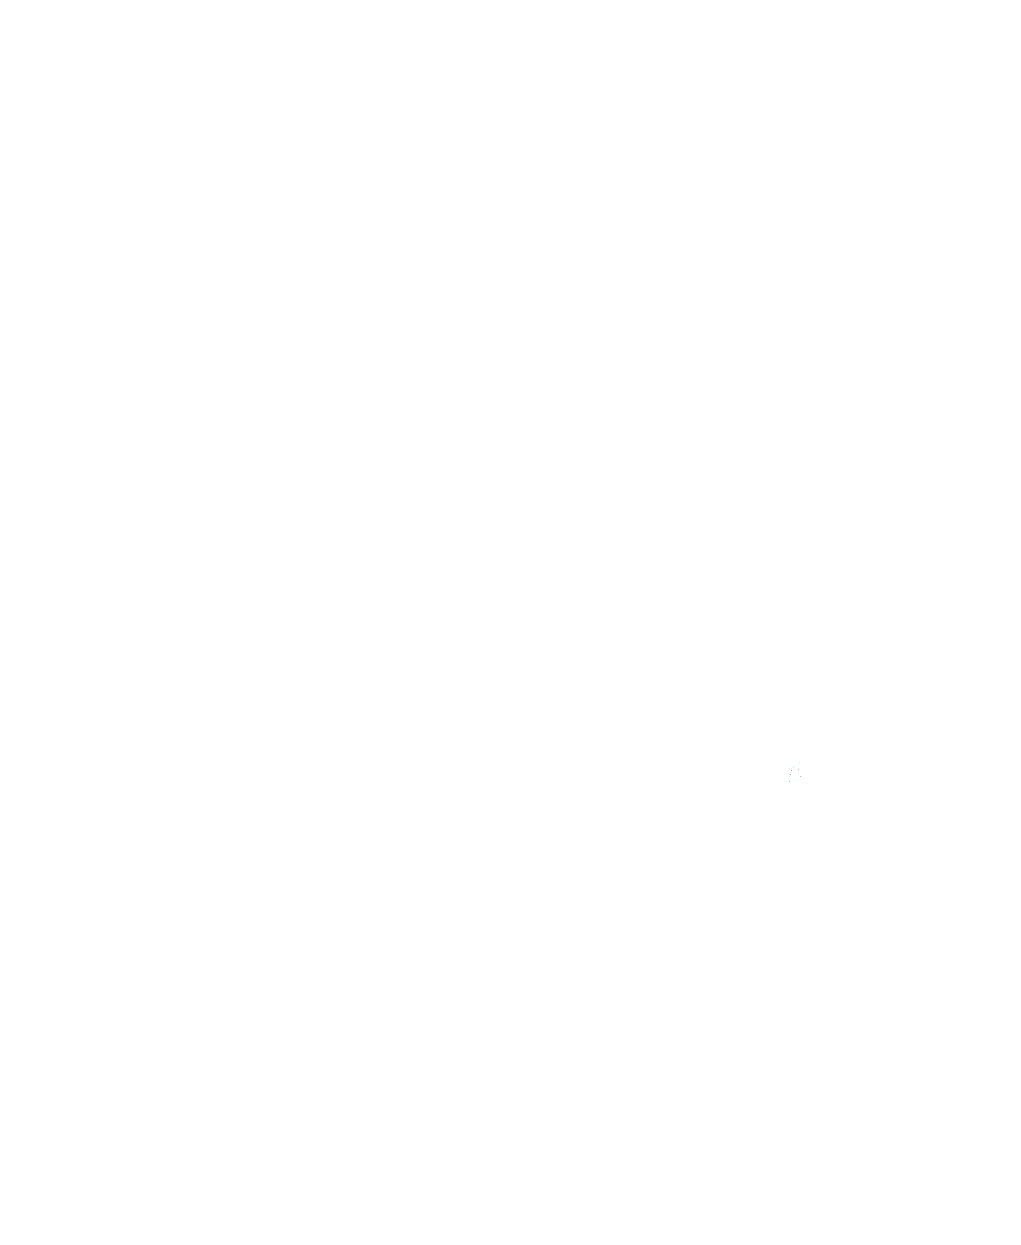
\includegraphics[width=\paperwidth,height=\paperheight]{../images/iris3.png}};
       \clearpage

  \begin{columns}
    \begin{column}{.5\textwidth}

    \end{column}
    \begin{column}{.5\textwidth}

    \end{column}
    \end{columns}

\end{frame}

%%%%%%%%%%%%%%
%% TEMPLATE
%%%%%%%%%%%%%%
%% \begin{frame}{\theframenumber. }
%%   \begin{columns}
%%     \begin{column}{.5\textwidth}

%%     \end{column}
%%     \begin{column}{.5\textwidth}

%%     \end{column}
%%     \end{columns}

%% \end{frame}


\begin{frame}{\theframenumber. Low-Hanging Fruit \& its Consequences for Diversity}


  \tikz[remember picture,overlay]
  \node[opacity=0.2, inner sep=0pt] at (current page.center)
       {
\includegraphics[width=\paperwidth,height=\paperheight]{../images/Low-Hanging-Fruit-Layered.png}};
       \clearpage

  \begin{columns}
    \begin{column}{.5\textwidth}
      \begin{itemize}
      \item A challenge facing any machine learning technique is to
      avoid getting trapped in merely \emph{local} optima.

      \item This can happen, for example, if
        it hyperspecializes on a particularly simple portion 
        -- the ``low hanging fruit'' -- of the problem set,
        while failing to adapt to more difficult problems.

      \end{itemize}
    \end{column}
    \begin{column}{.5\textwidth}
      \begin{itemize}
      \item The phenomenon is analogous to a natural population
        over-adapting to a particularly hospitable niche.
      \item But in the wild, this is
        offset by an increase in competition and crowding,
        which increase the selective pressure acting on formerly
        hospitable niches. Low-hanging fruit doesn't last very long.
      \end{itemize}
    \end{column}
    \end{columns}
\end{frame}



\begin{frame}{\theframenumber. Implementing Niching through Fitness Sharing}
  \begin{columns}
    \begin{column}{.5\textwidth}
      \begin{itemize}
      \item In order to address this issue, we first need to keep track of where, in the problem space, the overfitting occurs. Where is the low-hanging fruit?
      \item To do this, we tag each problem in our space with a `difficulty' field, which keeps track of how our specimens perform on it, on average. 
      \end{itemize}
    \end{column}
    \begin{column}{.5\textwidth}
      \begin{itemize}
      \item Since the whole point of tracking difficulty is to have it transform dynamically over the course of the evolution, we'll update these scores every so many iterations.
      \item On the next slide, we plot the progress of the population's best and average fitness scores on the left, and the difficulty rations of our problems on the right -- plotted by class mean and standard deviation. 
      \end{itemize}

    \end{column}
    \end{columns}
\end{frame}

\begin{frame}{\theframenumber. Tracking Niches without Crowding}
  \begin{center}
    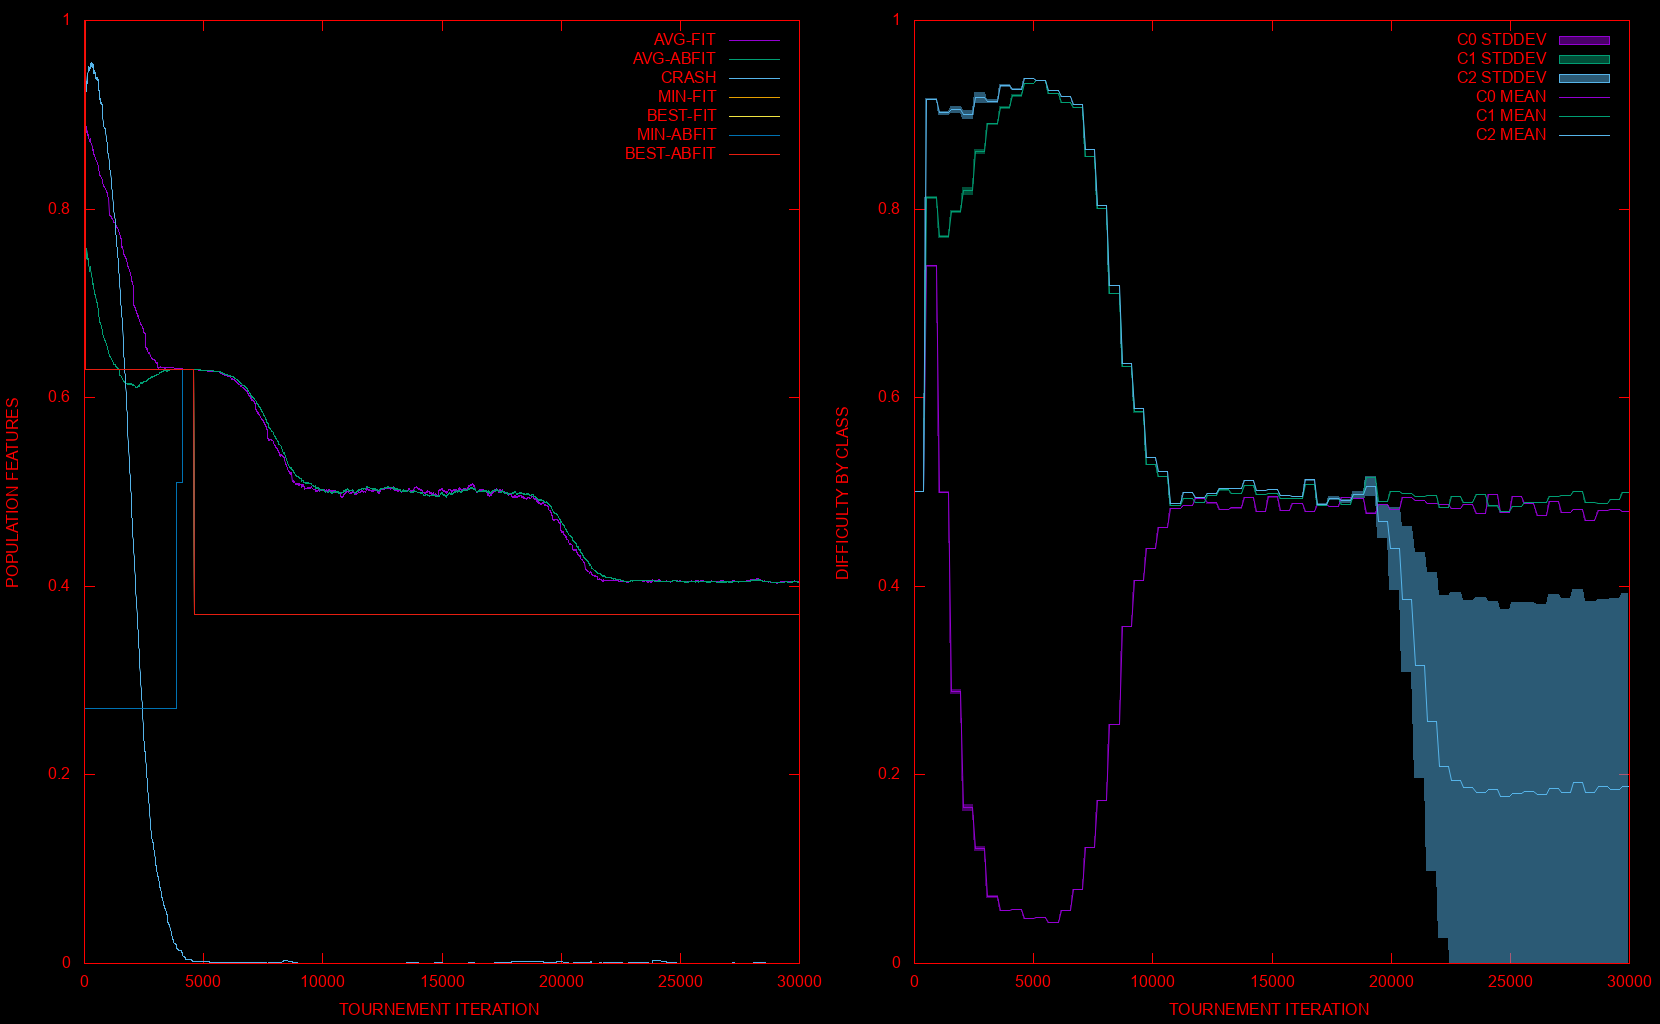
\includegraphics[width=\textwidth, height=.85\textheight]{../../examples/iris/nosharing-diff/nosharing.png}
  \end{center}
\end{frame}

\begin{frame}{\theframenumber. Crowding Implemented as Fitness Sharing}
  \begin{columns}
    \begin{column}{.5\textwidth}
      \begin{itemize}
      \item We haven't yet changed anything in the way each specimen's fitness is evaluated. The graph only shows us how the population is performing, with respect to each class of problems.
      \item But we can use this information to tweak our fitness function in ways relevant to niching.
      \end{itemize}
    \end{column}
    \begin{column}{.5\textwidth}
      \begin{itemize}
      \item All that we need to do is to scale the fitness points awareded for each problem with respect to that problem's difficulty. The rewards for solving `difficult' problems (uncrowded niches) will be greater than those awarded for solving `easy' problems (crowded niches). 
      \end{itemize}
    \end{column}
    \end{columns}

\end{frame}

\begin{frame}{\theframenumber. Niching with Crowding}
  \begin{center}
  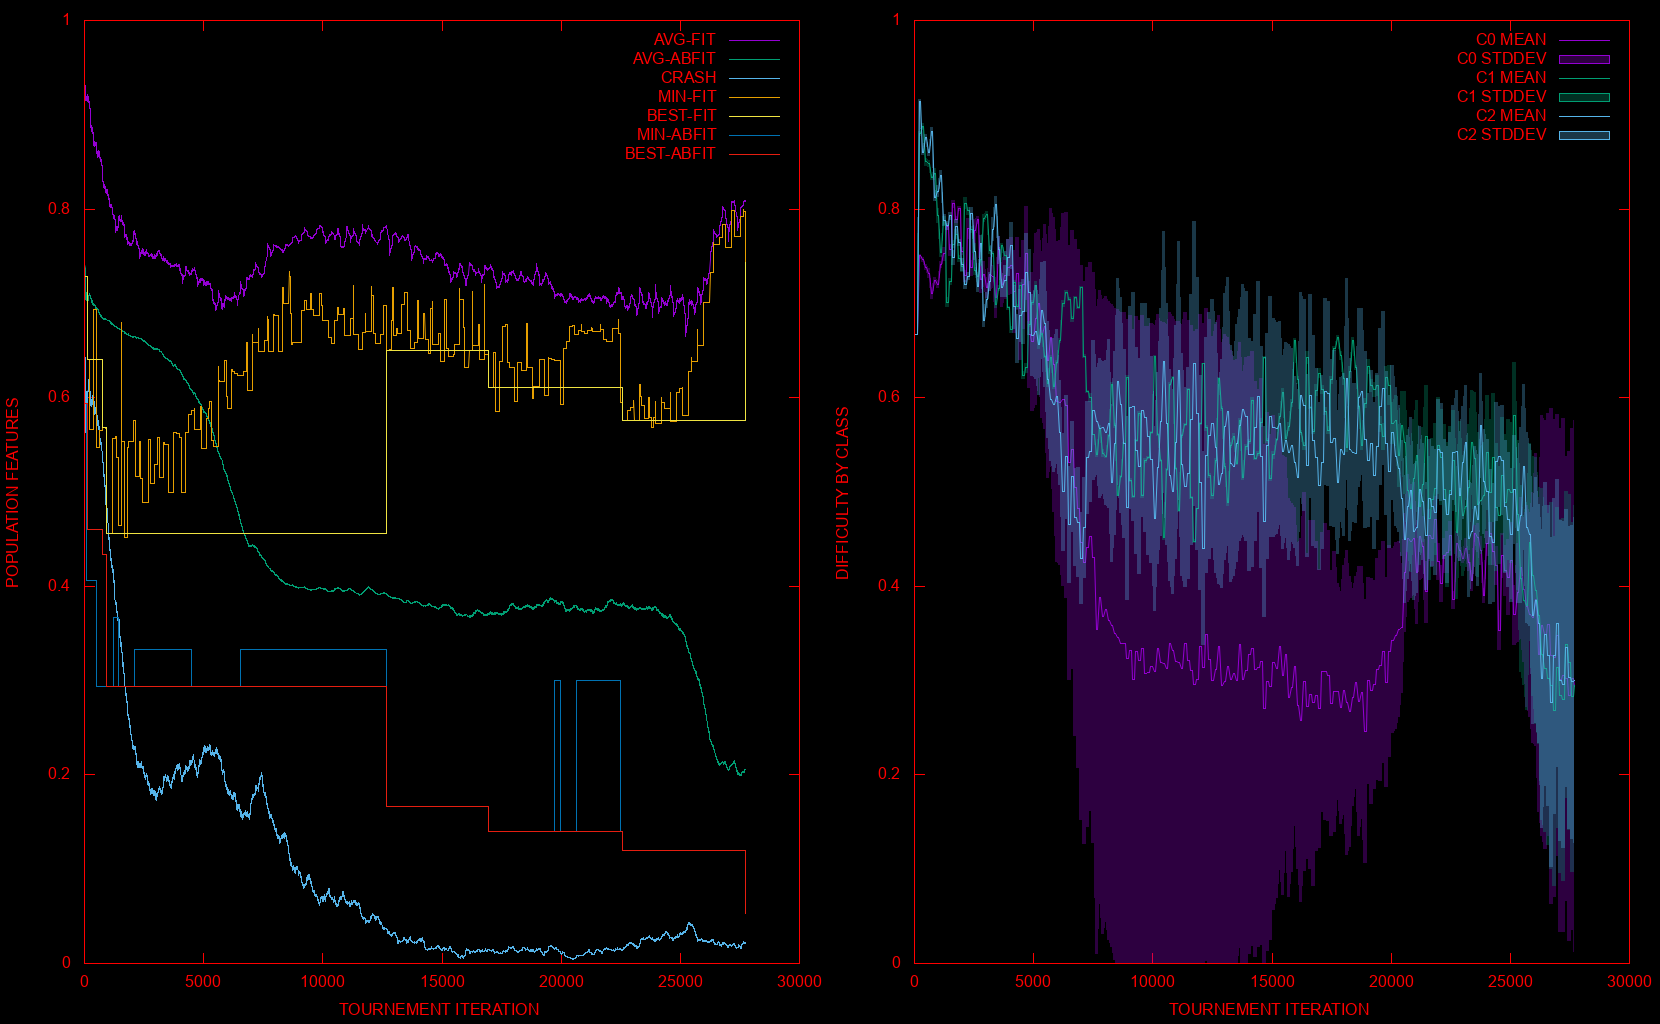
\includegraphics[width=\textwidth, height=.85\textheight]{../../examples/iris/sharing3/sharing3-black.png}
  \end{center}
\end{frame}

\begin{frame}{\theframenumber. Dynamic Braiding of Difficulty by Niche}
  \begin{figure}
    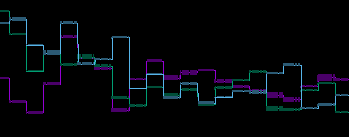
\includegraphics[width=\textwidth]{../images/braiding.png}
  \end{figure}
  A detailed view of the intricate braiding of niche availability that takes place once we enable fitness sharing. The image is an enlargement of the right panel of the graph on the last slide, focussing on the region between iterations 3000 and 5000.
\vspace{8pt}

  Because the environment perennially adjusts to the population's strengths and weaknesses, no specimen encounters the exact same fitness space as its distant ancestors, and cannot benefit from overfitting, or a diet of exclusively low-hanging fruit.
\end{frame}

\end{document}

%%%%%%%%%%%%%%
%% TEMPLATE
%%%%%%%%%%%%%%
%% \begin{frame}{\theframenumber. }
%%   \begin{columns}
%%     \begin{column}{.5\textwidth}

%%     \end{column}
%%     \begin{column}{.5\textwidth}

%%     \end{column}
%%     \end{columns}

%% \end{frame}
